\documentclass{beamer}
\usepackage{hyperref}
\hypersetup{unicode=true}
\usepackage[utf8x]{inputenc}
\usepackage[english,russian]{babel}
\usepackage{beamerthemesplit}
\graphicspath{{pics/}}


\usepackage{color}
\definecolor{gray}{rgb}{0.4,0.4,0.4}
\definecolor{bggray}{rgb}{0.9,0.9,0.9}
%	Параметры подсветки исходного кода на C++
\usepackage{listings}
\lstset{breakatwhitespace,
	language=C++,
	columns=fullflexible,
	keepspaces,
	breaklines,
	tabsize=3,
	numbers=left, % нумерация строк
	numberstyle=\small\color{gray},
	numbersep=5pt,
	backgroundcolor=\color{bggray},
	showstringspaces=false,
	extendedchars=true,
	keywordstyle=\color{blue}\ttfamily,
	stringstyle=\color{red}\ttfamily,
	commentstyle=\color{green}\ttfamily,
	morecomment=[l][\color{magenta}]{\#}
}


\begin{document}
\title[Численные методы акустооптики на C++]{Отчёт о ведении спецкурса \\"Численные методы в приложении к задачам акустооптики и акустоэлектроники на языке программирования С++" в 2012 году}
\author{Арсений Трушин \& \(Co\)} 
\date{\today}

%% %	Пример листинга на C++, отступы, включая отступы от начала строки сохраняются (!)
%% \defverbatim[colored]\lst{
%%   \begin{lstlisting}[tabsize=2,basicstyle=\ttfamily]
%%     const char *processing() const{
%%       somestring = "-1";
%%     }
%% \end{lstlisting}}

%% %	Вставка листинга на C++
%% \frametitle{Пример кода на C++}
%% \lst

%	Слайд-заголовок (#1)
\frame{\titlepage}
%	Слайд с содержанием презентации (#2)
\frame{\frametitle{Содержание}\tableofcontents} 

\section{Обзор. Цели и методы спецкурса.}
\subsection{Проблема}
\frame{
  \frametitle{Преподавание программирования на Физфаке}
  \begin{block}{Первые курсы}
    \begin{itemize}
    \item На первых курсах есть C++
    \item Рассказывают о Win32API
    \item Не рассказывают о STL
    \end{itemize}
  \end{block}
  \begin{block}{В рамках спецкурса}
    \begin{itemize}
    \item Решение практических задач
    \item ``Точки входа'' в полезные технологии
    \item Решения в ``две строчки''
    \end{itemize}
  \end{block}
}
%
\subsection{Предлагаемое решение}
\frame{
  \frametitle{Особенности спецкурса}
  \begin{block}{Организационные}
    \begin{itemize}
    \item Маленькая группа - адаптивность
    \item Нацеленность на актуальные задачи
    \end{itemize}
  \end{block}
%
  \begin{block}{Технологии}
    \begin{itemize}
      \item g++/mingw
      \item emacs
      \item git
      \item povray
    \end{itemize}
  \end{block}
}
%
\section{Рассмотренные задачи и инструменты}
\subsection{Подбор констант для кристалла ниобата лития}
\subsubsection{Уравнения Кристоффеля для ниобата лития}

\begin{frame}{Уравнения эластодинамики для пьезоэлектрика}
	
\begin{columns}
\column{7 cm}
	\begin{block}{Уравнения Кристоффеля:}

\ $\Gamma_{il} p_l = \rho V^2 p_i$\\

\ $\Gamma_{il} = \bar{c}_{ijkl} n_j n_k$ -- компоненты тензора Кристоффеля

\ $\lambda=\rho V^2$

  \end{block}
	
  \begin{block}{Пьезоэффект:}
	
\ $\bar{c}_{ijkl} = c_{ijkl}^E + (e_{pij} n_{p}) (e_{qhl} n_{q}) / \epsilon_{jk}^S n_{j} n_{k}$

\ $e_{pij}, e_{qhl}$ -- пьезоэлектрические модули

\ $\epsilon_{jk}^S$ -- диэлектрическая проницаемость

  \end{block}
	
\column{5 cm}
	
\begin{figure}

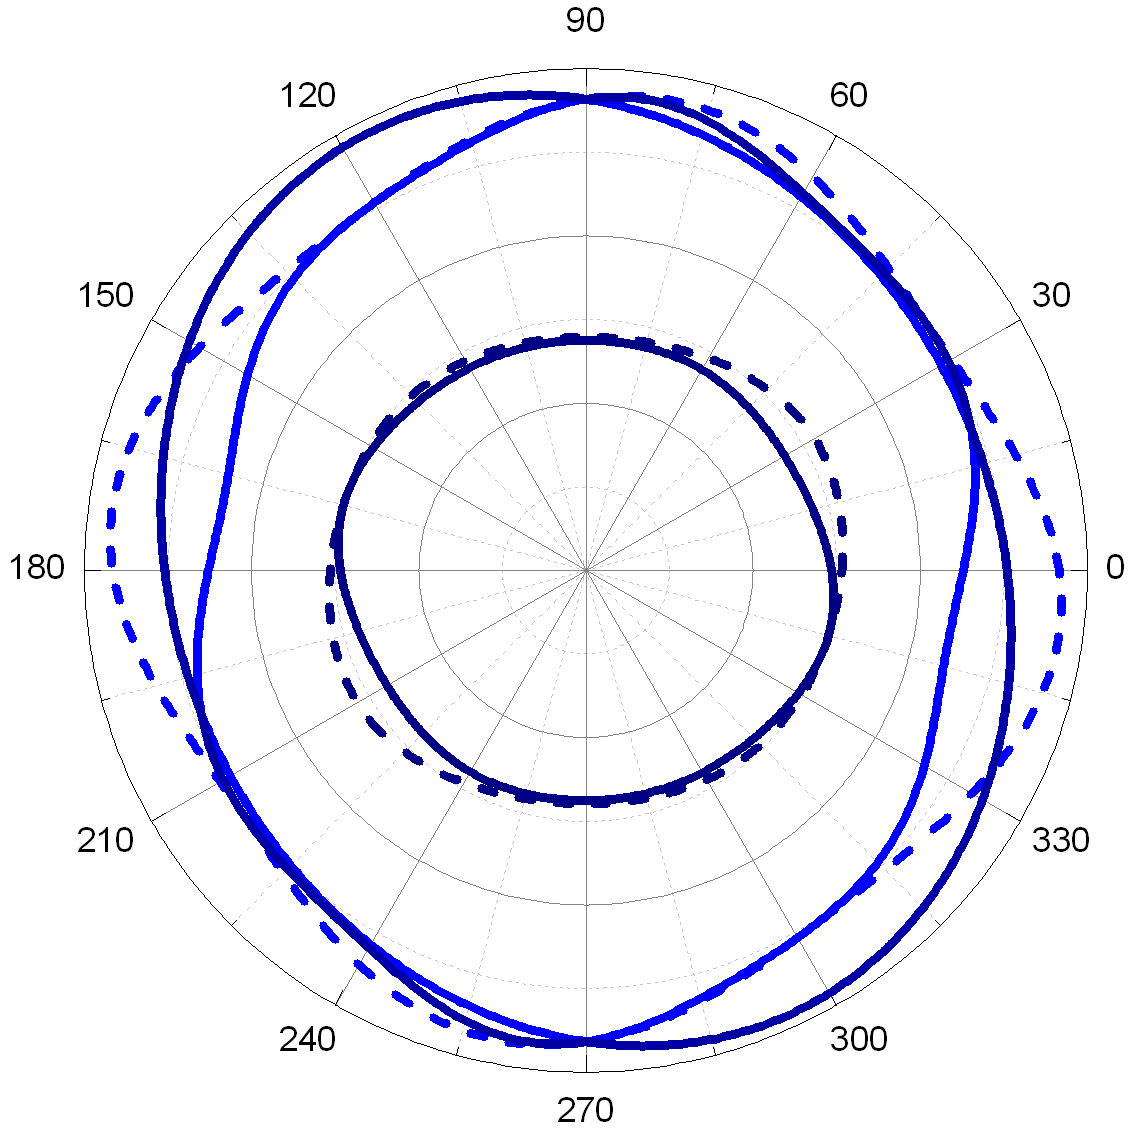
\includegraphics[width=5 cm]{linbo3_piezo.png}

\end{figure}

\end{columns}
\end{frame}

%
\subsubsection{Использование PovRay для визуализации результатов расчёта}
\frame{ 
  \frametitle{Поверхность медленности ниобата лития}
  Никита
}
%
\subsubsection{Экстракция экспериментальных данных}
\frame{
  \frametitle{Проблемы извлечения данных}
  \begin{columns}
    \column{6 cm}
    \begin{figure}
      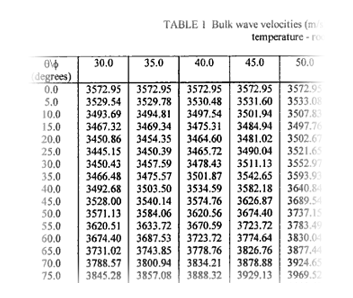
\includegraphics[width = 6cm]{table_example.png}
    \end{figure}
    \column{7 cm}
    \begin{table}
      \begin{tabular}{ c  c  c  c }
        \hline 
        \theta \backslash \varphi & 30.0 & 35.0 & 40.0 \\
        \hline
        0.0  & 3572.95 & 3572.95 & 3572.95 \\
        5.0  & 3529.54 & 3529.78 & 3530.48 \\
        10.0 & 3493.69 & 3494.81 & 3497.54 \\
        15.0 & 3467.32 & 3469.34 & 3475.31 \\
        \hline
      \end{tabular}
    \end{table}
  \end{columns}
  Здесь должна быть ссылка на литературу
}
\frame{
  \frametitle{Проблемы извлечения данных}
   \begin{block}{Шаги подготовки данных}
    \begin{itemize}
      \item Перевод данных из графического в тестовый вид \\ {\hspace{6 cm} \footnotesize{OCR программы}}

      \item Считывание данных из txt в основную программу

      \item Устранение ошибок распознавания \\ {\hspace{6 cm} \footnotesize{B542,\% $\rightarrow$ 8542.96}}

      \item Поиск численных ошибок по величине невязки \\ {\hspace{6 cm} \footnotesize{8542.96 $\rightarrow$ 3542.96}}
    \end{itemize}
  \end{block}
}

%
\subsubsection{Метод отжига}
\frame{
  \frametitle{Метод отжига}
  \begin{block}{Начальные условия}
    \begin{itemize}
      \item Начальный набор констант $\{c^0_{ijkl}\}, \{e^0_{pij}\}, \{\epsilon^0_{jk}\}$ из Кушибики
      \item Экспериментальные значения скоростей $V_i(\phi, \theta)$ Книжка 
    \end{itemize}
  \end{block}
  \begin{block}{Хотим}
    \begin{itemize}
      \item Получить набор констант $\{c_{ijkl}\}, \{e_{pij}\}, \{\epsilon_{jk}\}$ дающий скорости максимально близкие к экспериментальным
    \end{itemize}
  \end{block}
}
\frame{
  \frametitle{Метод отжига}
  \begin{columns}
    \column{7 cm}
      \begin{itemize}
      \item Случайно выбираем параметр из $\{c^0_{ijkl}\}, \{e^0_{pij}\}, \{\epsilon^0_{jk}\}$, изменяем его на $\delta(T)$, расчитываем текущие скорости
      \item Считаем невязку текущих и экспериментальных скоростей $\Delta^{curr}$
      \item Если $\exp(-\frac{\Delta^{curr}-\Delta^{best}}{T}) > rand() \Rightarrow$ запоминаем текущие параметры как лучшие
%$\Delta^{curr} \rightarrow \Delta^{best}$; $V^{curr} \rightarrow V^$
      \item Повторяем пока не получим желаемый $\Delta^{best}$
      \end{itemize}
    \column{5 cm}
    \begin{figure}
      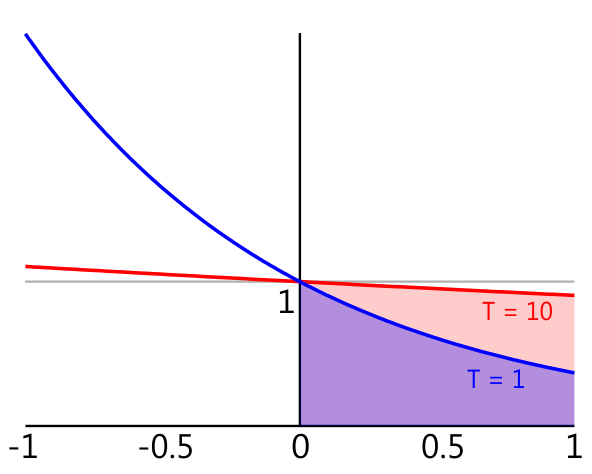
\includegraphics[width = 5cm]{exponent.png}
    \end{figure}
  \end{columns}



}
%
\subsubsection{Рой}
\frame{
  \frametitle{Рой}
  Никита
}
\subsection{PovRay}
\frame{
  Уже говорилось, что PovRay - это удобный инструмент для визуализиции результатов расчёта, кроме того, он позволяет делать 
  трёхмерные иллюстрации и мультфильмы. Пример кода и что из него получается.
  
  Полина
}
\subsection{Дифракция методом Фурье}
\frame{ 
  \frametitle{Дифракция на щели}
  
  Решение задачи о дифракции света на щели с использованием двумерного преобразования Фурье
  
  Дима
}
%

%Мобилограмма
% Tools:
% - C++ (С)
% - Qt (С)
% - mingw (С)
% - emacs (С)
% - git (С)
% - PovRay (П)
% Подбор констант:
% - кристоффель (Ю)
% - экстракция скоростей из файла (Ю)
% - градиентный спуск (П)
% - рой (Н)
% - отжиг (С)
% - дифракция (Д)

%\section{Подбор констант}
%\subsection{Метод отжига}\frame{}
%\subsection{Градиентный спуск}\frame{}
%\subsection{``Рой''}\frame{}

%\frame{
%\subsection{сПиСоК}
%\frame{\frametitle{unnumbered lists}
%\begin{itemize}
%\item Как выстрелить себе в ногу при помощи C++ и \LaTeX  
%\item *Курс для продвинутых
%\item Быдлокод
%\item BDD, TDD, Agile, XP и другие страшные слова
%\end{itemize} 
%}
%
%\frame{\frametitle{lists with pause}
%\begin{itemize}
%\item Introduction to  \LaTeX \pause 
%\item Course 2 \pause 
%\item Termpapers and presentations with \LaTeX \pause 
%\item Beamer class
%\end{itemize} 
%}
%
%\subsection{Lists II}
%\frame{\frametitle{numbered lists}
%\begin{enumerate}
%\item Introduction to  \LaTeX  
%\item Course 2 
%\item Termpapers and presentations with \LaTeX 
%\item Beamer class
%\end{enumerate}
%}
%\frame{\frametitle{numbered lists with pause}
%\begin{enumerate}
%\item Introduction to  \LaTeX \pause 
%\item Course 2 \pause 
%\item Termpapers and presentations with \LaTeX \pause 
%\item Beamer class
%\end{enumerate}
%}

%\section{Section no.3} 
%\subsection{Tables}
%\frame{\frametitle{Tables}
%\begin{tabular}{|c|c|c|}
%\hline
%\textbf{Date} & \textbf{Instructor} & \textbf{Title} \\
%\hline
%WS 04/05 & Sascha Frank & First steps with  \LaTeX  \\
%\hline
%SS 05 & Sascha Frank & \LaTeX \ Course serial \\
%\hline
%\end{tabular}}
%
%
%\frame{\frametitle{Tables with pause}
%\begin{tabular}{c c c}
%A & B & C \\ 
%\pause 
%1 & 2 & 3 \\  
%\pause 
%A & B & C \\ 
%\end{tabular} }
%
%
%\section{Section no. 4}
%\subsection{blocs}
%\frame{\frametitle{blocs}
%
%\begin{block}{title of the bloc}
%bloc text
%\end{block}
%
%\begin{exampleblock}{title of the bloc}
%bloc text
%\end{exampleblock}
%
%
%\begin{alertblock}{title of the bloc}
%bloc text
%\end{alertblock}
%}
\end{document}

